\documentclass[11pt,a4paper]{article}
%\usepackage[toc,page]{appendix}
\usepackage{graphicx}
\usepackage[a4paper]{geometry}
\usepackage{xcolor}
\usepackage{fancyhdr}
\usepackage{float}
\usepackage{setspace}
\usepackage[absolute]{textpos}
\usepackage{epstopdf}
%\usepackage[]{mcode} 	% To include matlab code
\usepackage{capt-of}
\usepackage{enumerate}
\usepackage{lastpage}
\usepackage{booktabs}
\usepackage{longtable}
\usepackage{array}
\renewcommand{\arraystretch}{1.5}

\usepackage[english]{babel}
\usepackage[utf8]{inputenc}
\usepackage{amsmath}
\usepackage{amsfonts}
\usepackage{graphicx}
\usepackage[colorinlistoftodos]{todonotes}
\usepackage{algorithm}
\usepackage{algpseudocode}
\usepackage{caption}
\usepackage{amsmath}
\usepackage{algorithm}
%\usepackage[noend]{algpseudocode}
\makeatletter
\def\BState{\State\hskip-\ALG@thistlm}
\makeatother

\usepackage{amsmath}
\usepackage{amsfonts}
\usepackage{amssymb}
\usepackage{eurosym}

%Tables
\usepackage{multirow}

% Header
\setlength{\headheight}{30pt}
\newgeometry{top=2.5cm, bottom = 1.5cm, left=2cm, right=2cm}
\pagestyle{fancy} 
\lhead{\includegraphics[height=0.8cm]{figures/{tue_logo}.png}}
%\lfoot{Group 4 - ``CASE"-HENK}
\cfoot{~}
\rfoot{Page \thepage ~of \pageref{LastPage}}

\usepackage{cleveref}
% Change cleveref reference eq. to equation same for figure
\crefname{equation}{equation}{equations}
\crefname{figure}{figure}{figures}
\crefname{table}{table}{tables}

% Change Section numbering to Problem 1
%\renewcommand{\thesection}{Problem \arabic{section}.}

\begin{document}
%\begin{titlepage}
%\vspace*{100pt}
%\begin{figure}
%\centering
%\includegraphics[width=0.5\textwidth]{figures/TUelogozondertekst}
%\end{figure}
%\begin{center}
%{ \huge \bfseries 4AT100 Automotive Systems Engineering Project\\[0.4cm] }
%\textsc{\Large Concept Project Plan}\\[0.5cm]
%
%\end{center}
%
%\vfill
%
%\renewcommand{\arraystretch}{1}
%
%\begin{flushleft} \large
%\begin{tabular}{l}
%Project Coordinators:\\
%Dr.Ir. A. van de Mortel-Fronczak (Asia) \\
%Dr.Ir. I. Barosan (Ion) \\
%\end{tabular}
%\end{flushleft}
%
%\begin{flushleft} \large
%\begin{tabular}{l l l l}
%Tutor: & & & \\
%L. Kefalidis (Lazaros) & & & \\
%& & & \\
%Authors:\hspace{30mm} 	& \hspace{35mm}	& \hspace{55mm} 	    		& 			\\
%S. Forno (Simone) 		& ​0978942		& T. de Mor\'ee (Tim)			& 0944052 	\\
%R.M.A. Goris (Rob) 		& 0808822		& T.M.A. van de Wiel (Thijs)	​& 0824530 	\\
%B.S. Haarsma (Bouke) 	& 0751757​		& H. Wils (Hielke) 				& 0807014 	\\
%\end{tabular}
%\end{flushleft}
%
%\begin{flushleft} \large
%\begin{tabular}{l}
%MSc. Programme Automotive Technology \\
%Eindhoven University of Technology \\
%\end{tabular}
%\end{flushleft}
%
%\begin{flushleft} \large
%\begin{tabular}{l}
%\today \hspace{8.4cm} Group 4 ``CASE"-HENK \\
%\end{tabular}
%\end{flushleft}
%
%\renewcommand{\arraystretch}{1.5}
%
%\end{titlepage}

\newgeometry{top=2.5cm, bottom = 3cm, left=2cm, right=2cm}

%\newpage
%
%\setcounter{tocdepth}{2}
%
%\tableofcontents
%\newpage


%------------------------------------------------

\section{Short recap on previous updates} \label{sec:recap}

The previous update document generated from the 4 guiding questions, requirements, environment, deliverable and validation, which are the core structure of the work. Based on this 4 points I am going to describe the changes we discussed during the last weeks, according to my progresses and according to mine and Jonas new findings on the topic. I am going to present here what has been $updated$, compared to the previous updates doc of 25.08. Changes do not substantially differ the work flow, some old workpackages have been removed or changed, to meet Jonas`s requirements, and to keep focused on the main goal of the work itself. A detailed \textbf{Gantt chart} attached to this email, shows the remaining work packages, with a concrete work timeline.
\vskip .2em
\textbf{What is new} \\
\textbf{The Requirements} did not substantially change from previous time, thus the deliverables are still affected on the filter parametrization. To see the first results of $GMapping$ params results see Section \ref{sec:results}. I am currently working to generate the second sets of parameters for our newly selected second localization method, a $Graphbased$ localization method. The third and last localization method is the $Wifii$ pure method, which is actually the main deliverable  for Jonas, the most interesting among all. He is very interested to see the results from this method; I still need to conduct some reserches on how to implement such a "remote" connection in ROS, and the strategies on where to insert Wireless tags in the Gazebo world. \\
\textbf{The Environment} The little Gazebo Arena environment (see updates 25.08 Figure 2) is still used as source to preliminary conduct filter testing. It has been already "GMapped" last time, and I recently tested the Amcl filter, which gives the robot`s poses given the previously Gmapped environment. More details and results are shown in the next Section. The end goal is however to translate those methods into a bigger and realistic environment, and test the filters there. Hence, the WZL production plant has been made with the Gazebo simulator; and also here more details are found below. The $Open$ and $Closed$ loops manouvres strategies changed slightly. The $Closedloop$ manouvre has been removed from the work-packages, seen as not an important source of validation for the results, and being part of another SLAM topic, called "end-to-end" point checking. The $Openloop$ strategy remains unchanged, thus for the filters validation we keep the same open loop paths. \\
\textbf{The Deliverables} are a set of localization trajectories, whose accuracies are dependent on the filter and Global and Local planner parametrization, but also the environment itself (i.e in the $Wifii$ case we expect that the localization performances are dependent on where the tags are placed). A preliminary results comparing trajectories is given in Section \ref{sec:results}. It is not clear, and this is still under discussion, whether the Amcl filter measurement model part (see Kirsch, Rohigh algorithm of updates 25.08) is going to be implemented as well. According to previous document, the original deliverable was this Rohig, Kirsch algorith; this changed in favour to a documented and parametrized analysis of different localization methods, which is also the Title of the work. As said in the above Requirements, the main interest for Jonas is to mainly see the results from the $Wifii$ localization plugin. \\
\textbf{The Validation} We validate the result by first find the sets of GMapping parameters of the Mapping phase (both for Amcl and Graphbased SLAM). This is fundamental since the Localizers strictly rely on the map performances created. This will be deeply showed in Section \ref{sec:results} below. For the Amcl now I found an optimal sets of tuned params for the WZL plant.
Once this is done, the Localizers are validated through only $Openloop$ drawn trajectories and a comparison can be carried out. \\
\vskip .2em
The next section shows concretely the obtained results of the above explained points.

\section{Updates and first results} \label{sec:results}

\textbf{The Global Planner implementation as ROS plugin} \\
In order to have a reproducible, standard test-path for our robot, a Global Planner has to be implemented in ROS. This consists of a simple path, first the robot drives 2meters forward and then makes a diagonal turn, as seen in Figure \ref{fig:planner}. This has been implemented for now only on the little MRL Arena environment first, but as seen, it works quite well. 
\begin{figure}[H]
	\center
	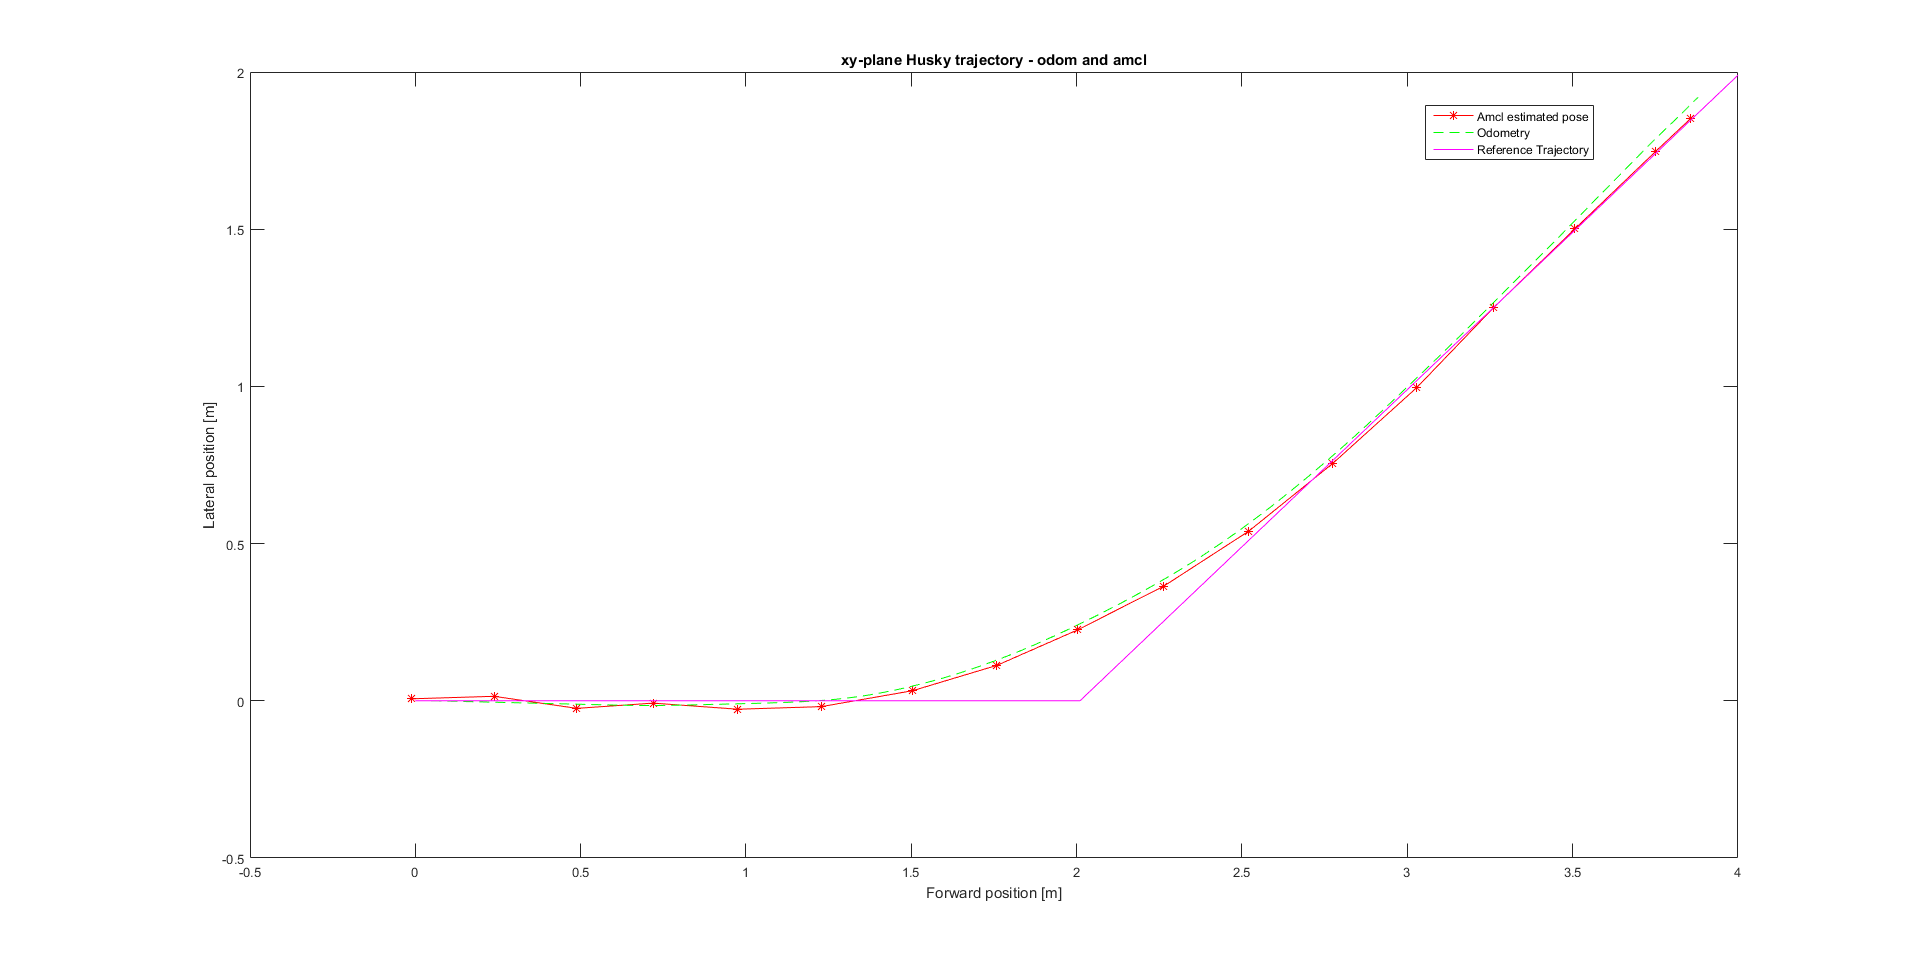
\includegraphics[width=1\textwidth]{figures/odom_amcl_ref.png}
	\caption{}
	\label{fig:planner}
\end{figure}

The pink trajectory is the base reference Planner path, path to which the robot sticks. In this Figure it is also visible the result from the Amcl filter in $red$, showing with an asterix, the estimated robot´s pose, spawn for this case as a frequency of 1 Hz. The green dotted line represents the wheel odometry instead. What will come next, which is not here jet, is also the $Graphbased$ estimate and the $Wifi$ estimate. \\
This simple Planner has been tested in the little MRL Arena environment for now, but we are pretty sure we won't have any troubles in making the same for the WZL big environment. 
\begin{figure}[H]
\minipage[t]{0.32\textwidth}
  \includegraphics[width=\linewidth]{figures/goal.png}
  \caption{The planner is tested by setting an arbitrary goal in the environment; this shouldn't coincise with the last point of the Planner. No matter where it is set, the robot sticks to the Planner path as soon as the goal is reached}\label{fig:goal}
\endminipage\hfill
\minipage[t]{0.32\textwidth}
  \includegraphics[width=\linewidth]{figures/start.png}
  \caption{The Planner path (pink) is drawn, particles are initialized and the robot starts to move}\label{fig:start}
\endminipage\hfill
\minipage[t]{0.32\textwidth}%
  \includegraphics[width=\linewidth]{figures/end.png}
  \caption{The robot reaches the goal}\label{fig:end}
\endminipage
\end{figure}

\vskip 1em
\textbf{Creation of the WZL model in Gazebo} \\
We leave the simple Arena environment to move to the final realistic one. We present here first the Gazebo model, then, as for the simple environment, we perform $Gmapping$. \\
The 2D plant and the 3D Gazebo reproduction can be viewed in Figure \ref{fig:WZL} and Figure \ref{fig:Gazebo}. The Gazebo model is in scale 1:1 with the 2D plant. \\
In the middle the environment presents highly simmetrical features, which are tricky for the filter and the localization. If the filter can withstand those situations, than it can be said to be robust enough. 
\begin{figure}[H]
    \centering
    \begin{minipage}[t]{.5\textwidth}
        \centering
        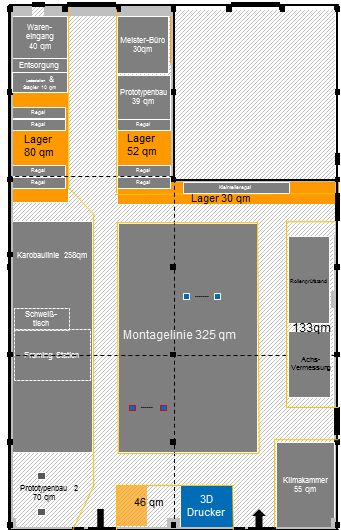
\includegraphics[width=0.7\linewidth, height=0.4\textheight]{figures/Layout_WZL}
        \caption{The 2D realistic environment plant}
        \label{fig:WZL}
    \end{minipage}%
    \begin{minipage}[t]{0.5\textwidth}
        \centering
        \includegraphics[width=0.7\linewidth, height=0.4\textheight]{figures/WZL_modif}
        \caption{The Gazebo 3D reproduction. In red the path the robot took to map the environment with $GMapping$; we found that the minimum path to sufficiently map the environment and have good results is the red one. To map the environment, the robot can avoid going into hidden spaces, as soon as the laser range is set to a proper value and heading (for the data see Table)}
        \label{fig:Gazebo}
    \end{minipage}
 \end{figure}

In Figure \ref{fig:Gazebo} we already sketched with a red line, the path the robot takes to perform $GMapping$, in details presented in the next section. \\

\textbf{GMapping} \\
The Amcl localization filter highly depends on the mapping quality of the environment in which the robot navigates. It is therefore necessary to find an \textbf{optimal} set of parameters, such that the mapping qualiy is good enough for localization. \\
The main $GMapping$ parameters are shown in Table \ref{tab:Table1}, together with the corresponding ROS and SLAM theory meaning. The bold parameters are the one which, according to [2] have the higher influence on the mapping performance, and therefore only those three were tuned. 

\vskip 2em
\begin{center}
\captionof{table}{GMapping default parameters} \label{tab:Table1}
\begin{tabular}{ | m{12em} | m{13cm}|} 
\hline
\textbf{Value} & \textbf{Explanation} \\ 
\hline
throttle{\_}scans=1 & Leave it as it is, according to [1] \\
\hline
map{\_}update{\_}interval=5 seconds & The time in seconds between map update, the lower the more frequent the map is updated, but comput costs are higher \\
\hline
maxUrange=29 maxRange=31 in meters & maxUrange less than laser range=30 meters \& maxRange higher than laser range.\\
\hline
sigma=0.05, lsigma=0.075 & Suitable definition still to be found\\
\hline
kernelSize=1 & has no unity, graphical window to look for scan matching correspondencies and applying ICP algorithm filter. Search window for the scan matching process \\
\hline
lstep and astep=0.05 & Initial search step in the scan matcher, I think it is similar to the ll/la sample range, but this is applied at the very first iteratin of the matcher \\
\hline
ogain=3 & gain to be used to smooth the resampling effect and likelihood \\
\hline
lskip=0 & number of scans skipped, might want to higher this and see whether the filter still is able to give good results \\
\hline
iterations=5 & the final precision of the scan matching is defined: precision = $lstep*2^(-iterations)$, the higher the number of iterations, the better the matcher precision \\
\hline
motion noise in general & A trade-off should be found in here, since the higher the noise, the more particles are needed to model the uncertainties. Best will be to found the minimum n. of particles with the highest possible noise \\
\hline
\textbf{linear=1 and angular update=0.5} & The robot processes scans after this value, an higher value might have an influence in the scan matcher performance (high computation cost in matching), or simply the filter skips some data \\
\hline
\textbf{resamplingThres=0.5} & the higher, the more frequent resampling occurs \\
\hline
\textbf{particles=100} & n.of filter particles \\
\hline
ll/lasamplerange=0.01 /step=0.005 & Range and steps are the spacing distance in sampling between points in the ICP algorithm of the scan matcher. As reference see slide see \textbf{Introduction to mobile robotics}. Lowering the range value takes more points to apply the minimization function of the ICP \\
\hline
occ{\_}thresh=0.25 & Highering this value might have an effect on the numbers of cell occupied, hence on the map performance, less cells can have the likelihood to be occupied! Occupied cell get the value 0, else -1 \\
\hline
xmin/max, ymin/max=-100/100 meters & initial map size  \\
\hline 
delta=0.05m (size of one cell) & Keep the same resolution \\
\hline
\end{tabular}
\end{center} 

\vskip 2em
We modified the three parameter above according to [2], with the values found in Table \ref{tab:Table2}, Table \ref{tab:Table3}  and Table \ref{tab:Table4}. \\

\textbf{Particle}

\begin{center}
\captionof{table}{GMapping default parameters} \label{tab:Table2}
\begin{tabular}{| m{12em} |} 
\hline
\textbf{Value} \\
\hline
particle=5 \\
\hline
particle=15  \\
\hline
particle=30  \\
\hline
particle=50  \\
\hline
\end{tabular}
\end{center}

\vskip 1cm

\textbf{Tuning the resampling threshold}

\begin{center}
\captionof{table}{GMapping default parameters} \label{tab:Table3}
\begin{tabular}{| m{12em} | m{13em}|} 
\hline
\textbf{Particles} & \textbf{ResThreshold} \\
\hline
particle=5 & Thr=0.1\\
\hline
particle=50 & Thr=1\\
\hline
particle=5 & Thr=1\\
\hline
particle=50 & Thr=0.1 \\
\hline
\end{tabular}
\end{center}

\textbf{Linear and angular update}

\begin{center}
\captionof{table}{GMapping default parameters} \label{tab:Table4}
\begin{tabular}{| m{12em} |} 
\hline
\textbf{Value} \\
\hline
linear=2 angular= 1  \\
\hline
linear= 4 angular=2  \\
\hline
linear= 8 angular=4  \\
\hline
linear=8 angular=4, particles=5   \\
\hline
\end{tabular}
\end{center}

The results in only changing the number of particles is shown in Figures \ref{fig:part5}, \ref{fig:part15}, \ref{fig:part50}. The maps look basically the same, hence no influence was found changing the particle number. The first reason for this result, might depend on the performance of the scan matcher, which is able to perfectly align scans with even 5 particles. A second reason for this is that the simulation has been run with a low speed (0.5 m/s), and the environment is highly regular. \\

\begin{figure}[H]
\minipage[t]{0.32\textwidth}
  \includegraphics[width=1\linewidth]{figures/p5.png}
  \caption{Five particles}\label{fig:part5}
\endminipage\hfill
\minipage[t]{0.32\textwidth}
  \includegraphics[width=1\linewidth]{figures/p15.png}
  \caption{Fifteen particles}\label{fig:part15}
\endminipage\hfill
\minipage[t]{0.32\textwidth}%
  \includegraphics[width=1\linewidth]{figures/p50.png}
  \caption{Fifty particles}\label{fig:part50}
\endminipage
\end{figure}

Combining particles with a different Resampling Threshold gave surprising effect. We would expect [2] errors in the constructed maps in the case of low particles and high resampling threshold. The results in Figure do not show this behavior. A proper justification for this should still be found, and it is probably also due to the one presented before. With an high number of particles, instead, the resampling effect vanishes. \\

% trying to put 4 figures as 2x2 matrix
\begin{figure}[H] \label{ fig7} 
  \begin{minipage}[b]{0.5\linewidth}
    \includegraphics[width=.8\linewidth]{figures/p5th1} 
    \caption{Particle 5, Resamplig Threshold 1} 
  \end{minipage} 
  \begin{minipage}[b]{0.5\linewidth}
    \includegraphics[width=.8\linewidth]{figures/p5th01} 
    \caption{Particle 5, Resamplig Threshold 0.1} 
  \end{minipage} 
  \begin{minipage}[b]{0.5\linewidth}
    \includegraphics[width=.8\linewidth]{figures/p50th1} 
    \caption{Particle 50, Resamplig Threshold 1} 
  \end{minipage}
  \hfill
  \begin{minipage}[b]{0.5\linewidth}
    \includegraphics[width=.8\linewidth]{figures/p50th01} 
    \caption{Particle 50, Resamplig Threshold 0.1}
  \end{minipage} 
\end{figure}

The linear and angulare updates play a relevant role in the scan matcher performance, hence on the mapping quality. In Figure we present what happens if the linear and angular updates are doubled. Also here, no difference has been found, and the matcher is able to align scans even if they are processed two times less than the default settings.

\begin{figure}[H] \label{ fig7} 
  \begin{minipage}[b]{0.5\linewidth}
    \includegraphics[width=.8\linewidth]{figures/l2a1} 
    \caption{Linear update 2 meters and angular updates 1 radiant} 
  \end{minipage} 
  \begin{minipage}[b]{0.5\linewidth}
    \includegraphics[width=.8\linewidth]{figures/l4a2} 
    \caption{Linear update 4 meters and angular updates 2 radiant} 
  \end{minipage} 
\end{figure}

Interestingly, Figure shows the effect of highering the motion noise, both in rotation and translation, from default values up to 10 times higher. The map looks completely distorted and cannot be used for navigation purposes. This confirms our expectations from the SLAM theory.

\begin{figure}[H] \label{ fig7} 
  \begin{minipage}[b]{0.5\linewidth}
    \includegraphics[width=.8\linewidth]{figures/motion_noise} 
    \caption{Effect of the motion noise} 
  \end{minipage}
\end{figure}
\vskip 2em

For the Amcl localization case, we found the optimum parameters set to be the default ones, changing only the number of particles to a minimum, for this case environment 5. We might want to "worsen" also other parameters, but we are happy with the map produced by the optimum set. \\
\textbf{What's next} \\
The detailed timeline of the remaining work packages is presented in the document Progress  Plan.xsl, attached on the email.
\section{References} \label{ref}

[1] ROS: http://wiki.ros.org/gmapping 
[2] A Quantitative Study of Tuning ROS Gmapping Parameters and Their Effect on Performing Indoor 2D SLAM, Yassin Abdelrasoul, Abu Bakar Sayuti HM Saman, Patrick Sebastian, Electrical and Electronic Engineering department Universiti Teknologi PETRONAS.




\end{document}



% == TABLE ==
%begin{table}[h!]
 % \centering
  %\caption{Caption for the table.}
 % \label{tab:table1}
 % \begin{tabular}{ccc}
 %   \toprule
  %  Some & actual & content\\
   % \midrule
   % prettifies & the & content\\
   % as & well & as\\
  %  using & the & booktabs package\\
  %   \bottomrule
  %\end{tabular}
%\end{table}


% === ALGORITHM == 

\iffalse % multi-comment tool
\begin{algorithm}[!h]
   \caption{Kirsch, Rohig algorithm}
    \begin{algorithmic}[1]
    	\State $St-1 = St$
        \For{$i = 1$ to $N$} \Comment{With N the number of particles in the filter set by maxparticle parameter}
            \State $Spread $ $particles$ $in$ $the$ $anchorbox$ $with$ $equations$ $1)$ $and$ $2)$ $of$ $[3]$ \Comment{This step is called $Global$ $Localization$}
            
            \State $xt[n] = p(xt|xt-1,ut)$ \Comment{Motion update - sample the particles from the motion update of the robot and move forward to estimate the error model functions}
            
        	\State $wt[n] = p(dnanoLOC|si)*p(dlaser|si)$ \Comment{Measurement update - si are the particles set with i the i-th index}
        	\State $St = St + <xt,wt>$ \Comment{add the state and weight to the total state space}
        	
        	\State $Perform$ $resampling$
        \EndFor
    \State $Return$ $St$

\end{algorithmic}
\end{algorithm}
\fi


\iffalse

\begin{figure}[!htb]
    \centering
    \begin{minipage}{.5\textwidth}
        \centering
        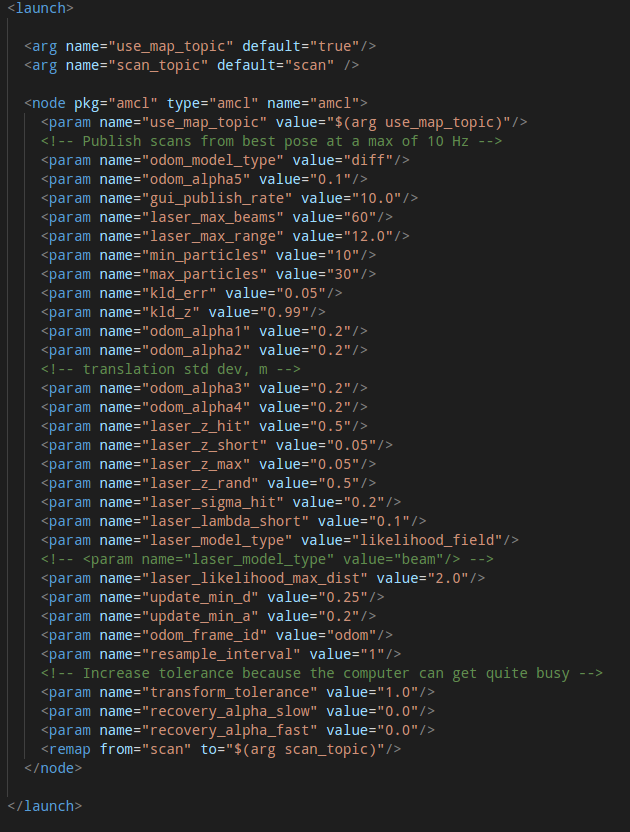
\includegraphics[width=0.7\linewidth, height=0.2\textheight]{figures/amcl_param}
        \caption{The $amcl$ tunable parameters}
        \label{fig:amcl_param}
    \end{minipage}%
    \begin{minipage}{0.5\textwidth}
        \centering
        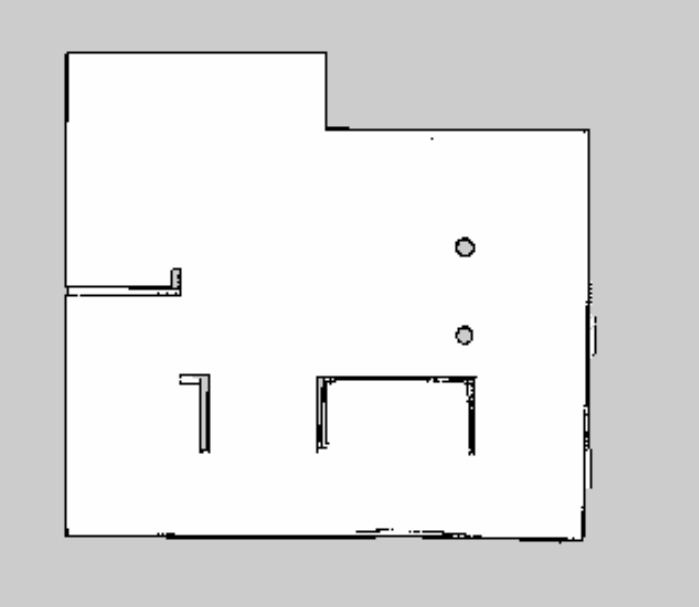
\includegraphics[width=0.7\linewidth, height=0.2\textheight]{figures/my_amcl_gmapping}
        \caption{Result of the Gmapping for the simple indoor environment}
        \label{fig:myamcl_map}
    \end{minipage}
 \end{figure}

% 3 column figure

\begin{figure}[H]
\minipage{0.32\textwidth}
  \includegraphics[width=\linewidth]{figures/goal.png}
  \caption{The planner is tested by setting an arbitrary goal in the environment; this shouldn't coincise with the last point of the Planner. No matter where it is set, the robot sticks to the Planner path as soon as the goal is reached}\label{fig:goal}
\endminipage\hfill
\minipage{0.32\textwidth}
  \includegraphics[width=\linewidth]{figures/start.png}
  \caption{The Planner path (pink) is drawn, particles are initialized and the robot starts to move}\label{fig:start}
\endminipage\hfill
\minipage{0.32\textwidth}%
  \includegraphics[width=\linewidth]{figures/end.png}
  \caption{The robot reaches the goal}\label{fig:end}
\endminipage
\end{figure}

 
 
 \begin{figure}[!htb]
	\center
	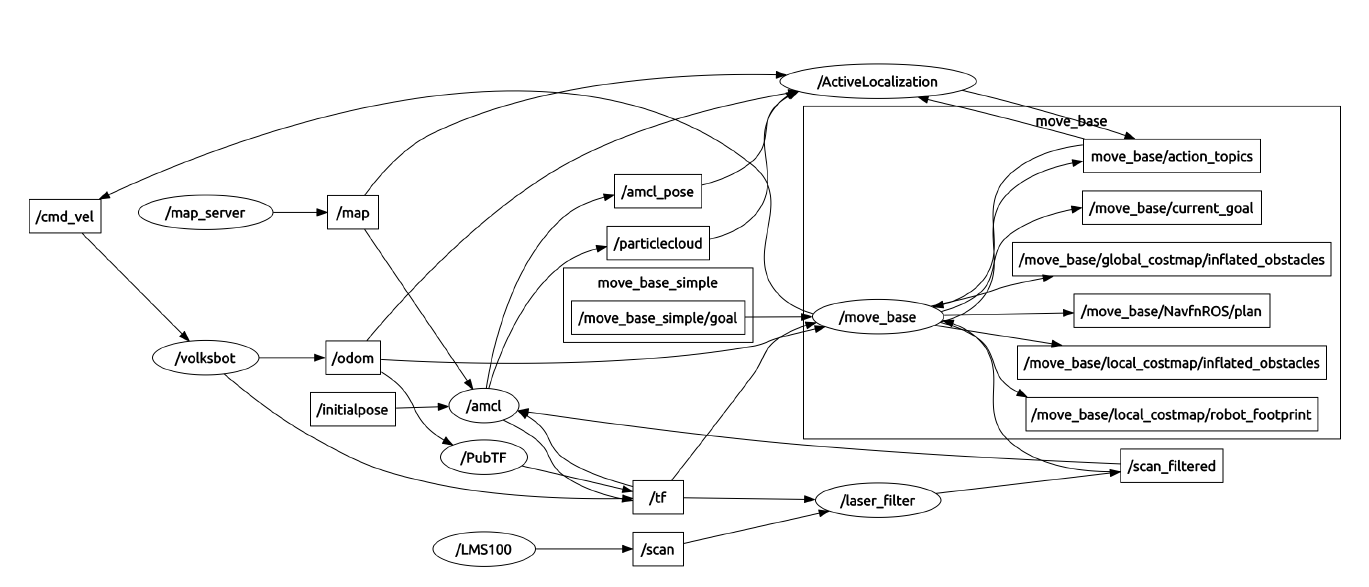
\includegraphics[width=1\textwidth]{figures/active_localization_node.png}
	\caption{An example of an active localization node}
	\label{fig:active_locnode}
\end{figure}


% underscore symbol {\_}


\fi